\begin{figure}[ht]
\centering
\scalebox{0.65}{%
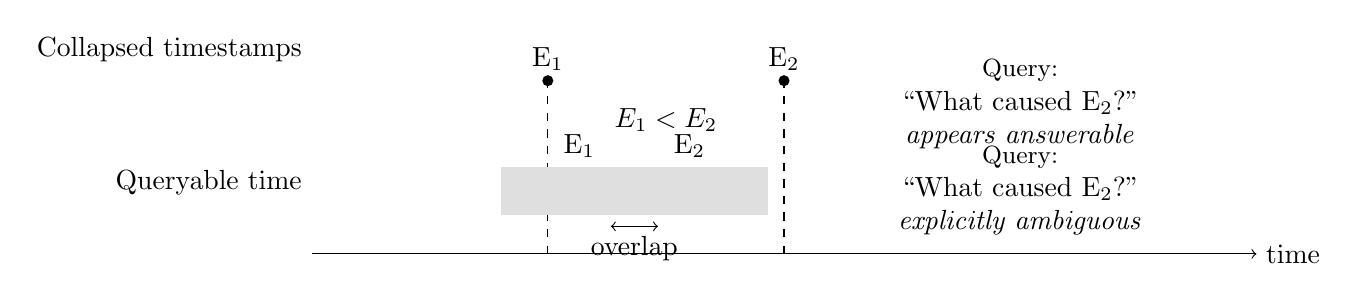
\begin{tikzpicture}[x=1cm,y=1cm]

% Time axis
\draw[->] (0,0) -- (12,0) node[right]{time};

% Labels
\node[anchor=east] at (0,2.6) {Collapsed timestamps};
\node[anchor=east] at (0,0.9) {Queryable time};

% ---- Collapsed case ----
% Events
\draw[dashed] (3,0) -- (3,2.2);
\fill (3,2.2) circle (2pt);
\node[above] at (3,2.2) {E$_1$};

\draw[dashed] (6,0) -- (6,2.2);
\fill (6,2.2) circle (2pt);
\node[above] at (6,2.2) {E$_2$};

% Forced ordering
\node at (4.5,1.7) {$E_1 < E_2$};

% Query annotation
\node[align=center] at (9,1.9)
  {\small Query:\\``What caused E$_2$?''\\\textit{appears answerable}};

% ---- Queryable case ----
% Event intervals
\draw[fill=gray!25,draw=none] (2.4,0.5) rectangle (4.4,1.1);
\node[above] at (3.4,1.1) {E$_1$};

\draw[fill=gray!25,draw=none] (3.8,0.5) rectangle (5.8,1.1);
\node[above] at (4.8,1.1) {E$_2$};

% Overlap marker
\draw[<->] (3.8,0.35) -- (4.4,0.35);
\node[below] at (4.1,0.35) {overlap};

% Query annotation
\node[align=center] at (9,0.8)
  {\small Query:\\``What caused E$_2$?''\\\textit{explicitly ambiguous}};

\end{tikzpicture}
}
\caption{Timestamp collapse versus queryable time. \conceptual\; When timestamps are collapsed to points (top), systems enforce a total ordering that makes causal queries appear answerable even when that ordering is unjustified; when temporal uncertainty is propagated (bottom), overlapping event intervals expose ambiguity, making causal queries explicit rather than silently wrong.}
\end{figure}